\documentclass[12pt,a4paper]{book}

               %%%%%%%%%%%%%%%%%%%%%%%%%%%%%%%%%%%%%%
               %    Scelta dei package da usare     %
               %%%%%%%%%%%%%%%%%%%%%%%%%%%%%%%%%%%%%%

\usepackage[italian]{babel}
\usepackage[latin1]{inputenc}
\usepackage{amsmath,amsfonts,amssymb,amsthm}
\usepackage{deistesi}
\usepackage{fancyhdr}
\usepackage{hyperref}
\usepackage{cleveref}
\usepackage{listings}
\usepackage{caption}
\usepackage{float}
\usepackage{wrapfig}
\usepackage{verbatim}
\usepackage{graphicx,subfigure}
\usepackage[nottoc]{tocbibind}
\floatstyle{boxed} % or whatever
\restylefloat{figure}
\captionsetup[lstlisting]{font={small,tt}}
               %%%%%%%%%%%%%%%%%%%%%%%%%%%%%%%%%%%%%%%%
               % Scelta delle dimensioni della pagina %
               %%%%%%%%%%%%%%%%%%%%%%%%%%%%%%%%%%%%%%%%

\setlength{\textwidth}{13.5cm}
\setlength{\textheight}{19cm}
\setlength{\footskip}{3cm}




               %%%%%%%%%%%%%%%%%%%%%%%%%%%%%%%%%%%%%%
               %  Informazioni generali sulla Tesi  %
               %    da usare nell'intestazione      %
               %%%%%%%%%%%%%%%%%%%%%%%%%%%%%%%%%%%%%%

\titolo{ADAS Ontology}
\laureando{Lorenzo Chiana}
\annoaccademico{2019--2020}
\facolta{CAMPUS DI CESENA\\SCUOLA DI INGEGNERIA}
\corsodilaurea{Ingegneria e Scienze Informatiche}
\corso{Web Semantico}
%\relatore{Alessandro Ricci}


\begin{document}

%%%%%%%%%%%%%%%%%%%%%%%%%
% inizio prefazione
%
% pagina del titolo, indice, sommario
%%%%%%%%%%%%%%%%%%%%%%%%%
\frontmatter
\maketitle
\pagestyle{plain} 
\tableofcontents
%``testo''


%%%%%%%%%%%%%%%%%%%%%%%%%
% inizio corpo del documento
%
% sequenze dei vari capitoli
% � consigliato mantenere una struttura logica ben definita per separare i vari capitoli
% si consiglia di reificare tale struttura fisicamente sul file system
%%%%%%%%%%%%%%%%%%%%%%%%%

\mainmatter

% stile della pagina
\pagestyle{fancy} \fancyhead[LE,RO]{\bfseries\thepage}

\chapter{Introduzione}

\section{Cause}

\index{Cause}

Al giorno d'oggi la costruzione di reti progettate per la condivisione ad alta capacit� di dati e il fatto che la comunicazione e la diffusione di concetti viene maggiormente veicolata attraverso l'uso di computer e di tecnologie simili, hanno permesso lo scambio sempre pi� crescente di dati governativi e commerciali mettendo, per�, in luce un problema fondamentale: la molteplicit� di lingue e di dizionari di dati.\\
Questo problema comporta un blocco del contenuto delle informazioni esistenti e connesse ad Internet e la mancanza di una lingua franca digitale � evidente nel dominio del cibo, poich� i materiali viaggiano dalla loro provenienza, agricola o meno, ai consumatori attraverso catene di processo e di distribuzione.\\
Un vocabolario bene definito e gerarchico, con relazioni logiche, ossia un'ontologia, � necessario per aiutare ad armonizzare quei dati che abbracciano i settori della sicurezza, qualit�, produzione e distribuzione alimentare e, di conseguenza, della salute e convenienza dei consumatori.

\section{FoodOn}

\index{FoodOn}

% inclusione dei capitoli
\chapter{FoodOn}

\section{Ontologia}
\index{Ontologia}
\section{Struttura}
\index{Struttura}
\section{Funzionalit�}
\index{Funzionalit�}


\chapter{Tecnologie}
In questo capitolo si vanno ad affrontare tutte le tecnologie utilizzate in questo progetto quali: RDF, RDFS, OWL, OWLAPI, SWRL, HermiT OWL Reasoner; dando anche una loro spiegazione.
\section{RDF}
\index{RDF}
Resource Description Framework o, abbreviato, RDF \`e lo strumento base proposto da W3C per la codifica, lo scambio e il riutilizzo di metadati strutturati che permette di descrivere le relazioni fra le entit\`a della parte di realt\`a che si vuole modellare.
In questa tecnologia l'unit\`a base per rappresentare l'informazione \`e lo \textit{statement}, ossia una tripla del tipo \textit{Soggetto - Predicato - Oggetto}.
In questa tripla il soggetto e l'oggetto rappresentano una risorsa e il predicato la relazione tra esse. \cite{rdf}

\begin{figure}[h!]
    \centering
    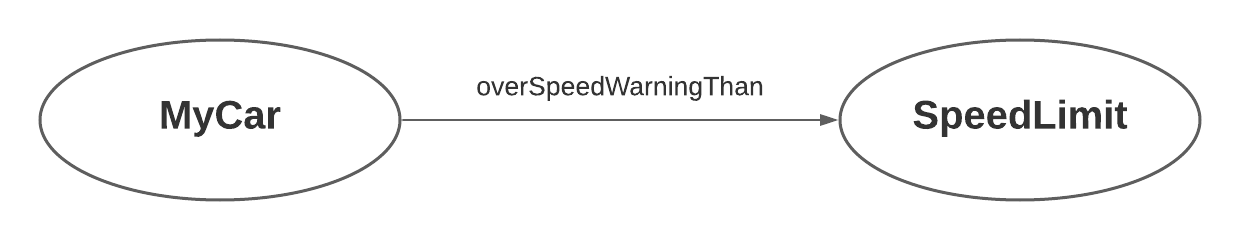
\includegraphics[width=0.90\textwidth]{img/overSpeedWarningThanRDF.png}
   	\caption{Tripla RDF con soggetto \textit{MyCar}, predicato \textit{overSpeedWarningThan} e oggetto \textit{SpeedLimit}}.
	\label{fig:triplaRDF}
\end{figure}

\section{RDFS}
\index{RDFS}
RDFS, acronimo di RDF Schema, \`e una tecnologia nata dall'esigenza di dover definire vocabolari e semantiche, cosa che non \`e possibile fare solo con RDF.
RDF Schema definisce un insieme di risorse RDF da usare per descrivere caratteristiche di altre risorse e propriet\`a RDF. \cite{rdfs}

\section{OWL}
\index{OWL}
OWL, acronimo di Web Ontology Language, \`e nato dall'esigenza di avere maggior potere espressivo rispetto a RDFS.
I componenti principali di un'ontologia OWL sono tre: individui, propriet\`a e classi. Gli individui rappresentano gli oggetti nel dominio di interesse, le propriet\`a sono relazioni binarie (ovvero che collegano due oggetti per volta) tra individui, le classi sono gruppi di individui.
\cite{owl}

\section{OWLAPI}
\index{OWLAPI}
OWLAPI \`e un'API per Java 8 nata per la creazione, la manipolazione e la serializzazione di ontologie OWL.
L'ultima versione si focalizza su OWL 2.
Vi \`e una ampia documentazione con tanto di esempi pratici nel loro repository (\url{https://github.com/owlcs/owlapi/wiki/Documentation}).

\section{SWRL}
\index{SWRL}
SWRL, acronico di Semantic Web Rule Language, \`e un linguaggio che consente la creazione di regole espresse in termini di concetti OWL (classi, propriet\`a, individuals).
Ci\`o fornisce una capacit\`a di ragionamento deduttivo pi\`u potente al solo utilizzo di OWL. 
SWRL supporta solo l'inferenza monotonica:
\begin{itemize}
\item le regole non possono essere utilizzate per modificare le informazioni esistenti in un'ontologia;
\item le regole non possono ritirare o rimuovere informazioni da un'ontologia.
\end{itemize}
Una regola SWRL \`e composta da una parte antecedente (il corpo) e da una parte conseguente (la testa), entrambi costituiti da congiunzioni positive di atomi.
Un atomo \`e espresso nella seguente forma: p(arg1, arg2, ..., argN) dove p \`e il simbolo del predicato e tra parentesi vi sono gli argomenti dell'espressione.\cite{swrl}

Esempi applicati al progetto:\\
\textbf{Mantenere una velocit\`a costante}\\
\begin{center}
\emph{isRunningOn(?X, ?Lane) $\char`\^$ OneWayLane(?Lane) $\char`\^$ SpeedLimit(?Y) $\char`\^$ overSpeedWarningThan(?X, ?Y) $\rightarrow$ constantSpeed(?X)}\\
\end{center}
In questo caso il body \`e rappresentato da tutto ci\`o che \`e antecedente alla freccia e la head da ci\`o che ne viene dopo.
Con questa regola il reasoner inferir\`a che se la head risulta vera allora anche il body lo sar\`a.
Nello specifico se esiste una tripla che:
\begin{enumerate}
\item associa le variabili \textit{X} e \textit{Lane} con la propriet\`a \textit{isRunningOn};
\item \textit{Lane} \`e istanza della classe \textit{OneWayLane};
\item \textit{Y} \`e istanza della classe \textit{SpeedLimit};
\item associa \textit{X} e \textit{Y} alla propriet\`a \textit{overSpeedWarningThan};
\end{enumerate}
allora \textit{X} deve mantenere una velocit\`a costante.\\
\textbf{Accelerare}\\
\begin{center}
\emph{isRunningOn(?X, ?Lane) $\char`\^$ OneWayLane(?Lane) $\rightarrow$ acceleration(?X)}\\
\end{center}
In questo caso la tripla che deve esistere per far s\`i che \textit{X} acceleri deve associare le variabili \textit{X} e \textit{Lane} con la propriet\`a \textit{isRunningOn} e che \textit{Lane} sia istanza di \textit{OneWayLane}.

\section{HermiT OWL Reasoner}
\index{HermiT}
HermiT \`e un reasoner per ontologie scritto in OWL.
Data una ontologia OWL HermiT \`e in grado di determinare se essa sia coerente o meno, identificare le relazioni di inclusione tra le classi e molto altro.
HermiT \`e il primo reasoner OWL disponibile pubblicamente basato sul nuovo calcolo ``hypertableau'' che fornisce un ragionamento molto pi\`u efficiente di qualsiasi algoritmo precedentemente noto. \cite{hermit}
Per i motivi sopracitati e per la grande disponibilit\`a di esempi trovati online anche, e soprattutto, dei vari esempi nella documentazione all'interno del Wiki del repository ufficiale di OWLAPI, la scelta del reasoner \`e ricaduta su HermiT.
\chapter{Conclusioni}
Questo progetto, che \`e in continua evoluzione, porta con s\'e un nuovo modello standard per la rappresentazione del cibo a livello mondiale che spazia da aspetti come la fonte, lo stato fisico e la forma; ad aspetti come l'origine culturale, processi di cottura, conservazione e trattamento, gruppo di consumatori e tipologia di prodotto.
La sua possibilit\`a di integrarsi con altri vocabolari semantici si rivela uno strumento chiave nel monitoraggio dei flussi di risorse e rifiuti tra sistemi antropogenici e naturali soprattutto nell'attuale era di crescente globalizzazione delle reti alimentari.
Inoltre, FoodOn si interessa anche dei recenti temi ambientali dati gli impatti del sistema alimentare umano sulla biodiversit\`a e sui servizi eco-sistemici. Per questo \`e stato progettato anche per essere interoperabile con ontologie incentrate sulla conoscenza ecologica, le pratiche agronomiche e lo sviluppo sostenibile.\\
Per le future release si prevede che la struttura tassonomica di classificazione di FoodOn sar\`a ulteriormente sviluppata per supportare la classificazione intuitiva degli alimenti e delle loro sfaccettature mantenendo, comunque, la coerenza con le ontologie correlate.\\
Un problema che l'attuale stato del progetto porta con s\'e riguarda ad alcune sfaccettature di LanguaL che contengono termini che possono essere ulteriormente definiti utilizzando una combinazione di nuove classi e classi gi\`a esistenti di altre ontologie.
Alcuni termini di FoodOn, probabilmente, saranno trasferiti ad altre ontologie consentendo, di conseguenza, di descrivere i database alimentari indicizzati con LanguaL gi\`a esistenti con componenti a maggior granularit\`a e di consentire a ragionatori di riconoscere membri appropriati di un tipo di prodotto alimentare e possibili componenti alimentari.
La granularit\`a per FoodOn \`e ancora un problema, basti pensare, ad esmpio, che la FAO elenca pi\`u di 12000 specie di pesci e molti di questi in FoodOn devono ancora essere importati e collegati all'uso culturale regionale.
Una possibile soluzione di questo problema per le prossime versioni del progetto \`e quella di incorporare le risorse che utilizzano gli standard del programma INFOODS\footnote{INFOODS  \`e una rete mondiale di esperti di composizione degli alimenti che mira a migliorare la qualit\`a, la disponibilit\`a, l'affidabilit\`a e l'uso dei dati sulla composizione degli alimenti.} della FAO.\\
Inoltre, in progetto c'\`e anche la possibilit\`a di andare ad esplorare la fattibilit\`a di un portale per la cura della terminologia, simil Wikipedia, che consente alle persone di suggerire definizioni o collegamenti a definizioni applicabili, sinonimi, riferimenti di tassonomia e riferimenti di immagini per termini per garantire un supporto migliore al multilingua e alla diversit\`a culturale.
Le varie proposte verranno poi supervisionate da un team che poi eventualmente le approver\`a.\\
La Hsiao Lab \`e, per ora, il principale curatore di FoodOn, ma l'ambizione globale del progetto dipende dall'attrazione diretta di nuovi partner e di una rete estesa di gruppi di lavoro IC3-FOODS\footnote{International Center for Food Ontology Operability Data and Semantics, consorzio internazionale che collabora con l'industria e i partner accademici di tutto il mondo per costruire una piattaforma semantica per l'IoF (Internet of Food).} attualmente in fase di organizzazione.\\
La struttura e il design di base del progetto ormai sono gi\`a stabili e ben definiti e ci\`o consente la partecipazione di organizzazioni private o pubbliche per aiutare a guidare, curare e fornire feedback sul suo sviluppo.
Attualmente il progetto FoodOn partecipa alla nuova discussione sull'armonizzazione dei sistemi di classificazione degli alimenti delle agenzie del gruppo di lavoro GODAN\footnote{Global Open Data for Agriculture and Nutrition o GODAN \`e un consorzio senza scopo di lucro finanziato da ONG e agenzie governative per l'alimentazione e la nutrizione.}.
Da ci\`o il progetto prevede l'emergere di un piano di sviluppo attuabile a lungo termine che includa sia i finanziamenti delle sovvenzioni stimolati dalla possibile diffusione del progetto, sia un modello di governance supportato dalla partecipazione a livello di agenzia.


%\appendix

% inclusione dei capitoli
%\chapter{FoodOn}

\section{Ontologia}
\index{Ontologia}
\section{Struttura}
\index{Struttura}
\section{Funzionalit�}
\index{Funzionalit�}



%%%%%%%%%%%%%%%%%%%%%%%%%
% inizio parte finale del documento
%
% eventuali appendici, bibliografia obbligatoria,
% eventuale lista delle tabelle e delle figure (nel caso decommentare la riga con i comandi \listoffigures e \listoftables)
%%%%%%%%%%%%%%%%%%%%%%%%%
\backmatter

\bibliographystyle{unsrt}
\bibliography{sample}


%\listoffigures
%\listoftables

% chiusura del documento
\end{document}
